% Is honesty one thing inside a language model?  Draft manuscript, 2026-10-31.
% Compiles with pdfLaTeX on Overleaf. Figures are in figures/ (drawn by cm/story_figs.py in the repository).
\documentclass[11pt]{article}
\usepackage[letterpaper,margin=1in]{geometry}
\usepackage[T1]{fontenc}
\usepackage[utf8]{inputenc}
\usepackage{newpxtext,newpxmath}
\usepackage{microtype}
\usepackage{graphicx}
\usepackage{booktabs}
\usepackage{tabularx}
\usepackage{array}
\usepackage{xcolor}
\usepackage{enumitem}
\usepackage{amsmath}
\usepackage[round,authoryear]{natbib}
\usepackage[font=small,labelfont=bf,labelsep=period,justification=justified,singlelinecheck=false]{caption}
\usepackage{titlesec}
\definecolor{accent}{HTML}{0B5F94}
\definecolor{muted}{HTML}{52514E}
\usepackage[colorlinks=true,allcolors=accent]{hyperref}

\titleformat{\section}{\large\bfseries}{\thesection}{0.8em}{}
\titleformat{\subsection}{\normalsize\bfseries}{\thesubsection}{0.8em}{}
\titlespacing*{\section}{0pt}{1.6em}{0.6em}
\titlespacing*{\subsection}{0pt}{1.2em}{0.4em}
\setlist{nosep,leftmargin=1.4em}
\setlength{\bibsep}{2pt}
\setlength{\emergencystretch}{1em}
\renewcommand{\arraystretch}{1.15}
\newcolumntype{L}{>{\raggedright\arraybackslash}X}

\renewcommand{\topfraction}{0.9}
\renewcommand{\bottomfraction}{0.6}
\renewcommand{\textfraction}{0.07}
\renewcommand{\floatpagefraction}{0.75}
\setcounter{topnumber}{2}
\setcounter{totalnumber}{3}

\newcommand{\gemma}{gemma-4-31b-it}
\newcommand{\qwen}{Qwen3.5-27B}
\newcommand{\cell}[2]{(#1, #2)}

\title{\vspace{-1.5em}Is honesty one thing inside a language model?\\[0.35em]
  \large Six definitions, four frames, and the distance between describing honesty and acting on it}
\author{Harsh Kumar\\ \small University of Toronto}
\date{\small Draft of 31 October 2026}

\begin{document}
\maketitle

\begin{abstract}
\noindent A model specification names a trait, such as honesty, and training and evaluation treat it as one thing:
one line in a constitution, one score on a benchmark, one direction to steer. Philosophy and psychology offer several
definitions of the same word, and virtue ethics adds that a trait has parts: perceiving, judging, acting, and a
self-conception. We ask whether honesty is one variable inside two instruction-tuned models, \gemma{} and \qwen{},
and if not, which part evaluations and training reach. We write six definitions of honesty as matched contrasts and
place each in four frames (recognize, judge, act, self-describe), 22 cells in all, read the residual stream in every
cell, and run nine downstream tasks that are consequences of honesty without being honesty evaluations. Where an
item sits in the model is set first by its frame; definition and polarity come second. A described-honesty variable
exists and generalizes across cells at two thirds of within-cell strength, most in self-description and least in
action. The models' failures are in conduct under pressure, not in the account they give of it afterwards; shown
their own covert cheating blind, they condemn it as readily as another model's, and they did it anyway. At the turn
where a model decides, its decision is decodable from the first layers on, and no described-honesty direction reads
it better than a random one. A prompt that licenses deception moves one model's conduct and its described-honesty
representation together, and the other model represents the licence without acting on it. Honesty, in these models,
is had and not used at the moment of acting: the akratic structure of Aristotle's account, shown on a system whose
internals can be read.
\end{abstract}

\section{Introduction}

Five premises fix the design, and the paper is their consequence.

\begin{enumerate}
\item \textbf{Model specifications name traits.} ``Be honest'' is one line in a constitution
  \citep{anthropic_constitution,openai_modelspec}, one number on a benchmark, one direction people steer. All three
  treat honesty as one thing.
\item \textbf{Philosophy and psychology do not.} \citet{williams2002} separates sincerity, asserting what one believes,
  from accuracy, taking care to believe truly. Calibration, knowing what one knows, is a third reading
  \citep{kadavath2022,li2024honesty}. Forthrightness, volunteering what matters, is a fourth. Non-sycophancy, holding
  the truth against the listener's wish, is a fifth \citep{sharma2023}. HEXACO honesty-humility, no manipulation and
  no entitlement, is a sixth \citep{ashton2007}. These are competing accounts of one named trait
  \citep{miller2021}, and each has a benchmark or a training recipe that targets it.
\item \textbf{A virtue has parts.} In virtue ethics a trait is not only conduct. It is perceiving what matters in a
  situation, judging well, choosing and acting, and a self-conception that holds the three together
  \citep{aristotle_ne,murdoch1970,mcdowell1979,blum1991,korsgaard1996}. When the parts come apart the names are old:
  akrasia when judgment is present and action does not follow \citep{davidson1970}, hypocrisy when self-description
  and action come apart \citep{batson1997}.
\item \textbf{Situations move conduct.} \citet{doris2002} and \citet{harmanG1999} argue from \citet{hartshorne1928}
  and \citet{milgram1963} that human conduct follows the situation more than the trait. For a model this is a test:
  the same model, a different pressure or a different system prompt, and we ask whether conduct moves while the trait
  readouts stay put.
\item \textbf{What ``one thing'' means inside a network.} If two things are one variable inside the model, a
  direction found for one reads the other, steering one moves the other, and both predict the same conduct. If none of
  that holds they are not one thing, whatever the word says.
\end{enumerate}

\noindent The question that follows: a trait named in a model specification, such as honesty, has several
definitions. Are they one thing inside the model? If not, which of them do evaluations and training reach?

\paragraph{Contributions.} (i) A design that crosses six definitions of honesty with four frames, with two
non-honesty controls that share the frame structure, run on two model families under one code path. (ii) A metric,
cross-context generalization of the honesty probe (leave-one-cell-out), with causal and behavioural validations.
(iii) A battery of nine tasks that are consequences of honesty without being honesty evaluations, with deterministic
cheat flags, a blind cross-judging protocol, an on-policy test of whether the honesty directions read the model's own
decisions, and a positive control. (iv) The finding that described honesty and the decision to act dishonestly are
carried by different variables, placed inside the philosophy and psychology of moral failure and read for what it
means for evaluation and character training.

\section{Background: a trait by its parts}

Once a trait has parts it can fail between them, and each failure has a literature. We use seven gaps
(Figure~\ref{fig:gaps}). The \emph{blind spot} is not seeing the moral dimension at all: \citet{gioia1992}, as Ford's
recall coordinator, twice voted against recalling the Pinto with the data in front of him and later wrote that his
scripts had no ethical component; \citet{tenbrunsel2004} call the mechanism ethical fading, \citet{bazerman2011}
bounded ethicality, \citet{bandura1999} moral disengagement; the philosophy of moral ignorance asks when it excuses
\citep{rosen2003,moodyadams1994,calhoun1989,wolf1987,zimmerman1997,fitzpatrick2008,harmanE2011}; Arendt's Eichmann
\citeyearpar{arendt1963,arendt1971} is the famous version and \citet{stangneth2014} the correction that the
performance in the dock was a performance. \emph{Akrasia} is judging rightly and acting otherwise: Socrates denied it
\citep{plato_protagoras}; Aristotle allowed it because knowledge can be had and not used, as the drunk recites
Empedocles \citep[VII.3]{aristotle_ne}; \citet{davidson1970}, \citet{hare1963} and \citet{holton2009} give the modern
forms; Milgram's subjects protested and continued \citep{milgram1963,milgram1974,burger2009}, and at J\'ozef\'ow about
a dozen of five hundred policemen took the offer to step out \citep{browning1992}, their revulsion showing that
perception and judgment were intact and the step to action was what failed \citep[contrast][]{goldhagen1996};
\citet{vaughan1996} gives the organizational form. \emph{Hypocrisy}, the say-do gap, is describing oneself one way
and acting another \citep{batson1997,batson1999,mazar2008,shalvi2011}, in its extreme form \citeauthor{lifton1986}'s
\citeyearpar{lifton1986} doubling. \emph{Self-leniency} is judging the same act more harshly in another than in
oneself \citep{valdesolo2007,valdesolo2008,monin2001}, and it is separable from the say-do gap. \emph{Concealment} is
hiding the act afterwards \citep{bok1978}, against owning it. \emph{Situation} is the same agent behaving differently
in a different setting \citep{hartshorne1928,burton1963,mischel1968,doris2002}. The inverse case, acting better than
one's judgment, is Huckleberry Finn \citep{bennett1974,arpaly2003} and the rescuers \citep{oliner1988,hallie1979,glover1999}.
The seventh gap, \emph{having without using}, is Aristotle's account turned into a measurement: if a system carries a
representation of the trait and that representation is not consulted when it decides, the knowledge is had and not
used, and a readable system lets us say so without inferring it from behaviour.

In language models, honesty has been surveyed as self-knowledge plus self-expression \citep{li2024honesty},
separated from accuracy \citep{ren2025mask,evans2021truthful}, and read from activations as truth or lie detectors
\citep{burns2022ccs,azaria2023,marks2023geometry,goldowskydill2025}. Character has been read as persona vectors
\citep{chen2025persona}, an assistant axis \citep{lu2026assistant}, a selected persona \citep{marks2026psm,danilov2026names},
and trained through constitutions \citep{maiya2025oct}. The probing literature supplies the distinction the paper
rests on, that a decodable property need not be a used one \citep{hewitt2019control,ravichander2021,elazar2021amnesic,belinkov2022},
and the steering literature its cautions \citep{wu2025axbench,galeone2026}. Behavioural work has found a knowledge-action
gap in models' stated and enacted values \citep{huang2026knowing}, omitted flaws in models' reports
\citep{huang2026insecure}, and proposed akrasia as the frame for agentic inconsistency \citep{yang2025akrasia}.
What we add is the internal side: the description and the decision are carried by different variables.

\section{Design}

\subsection{Definitions, frames, cells}

Six definitions of honesty, each a matched contrast: the same scenario in an honest and a dishonest version
(Table~\ref{tab:defs}). Each appears in four frames: the model's own reply about someone else's conduct (a,
recognize), its own reply on whether that conduct was acceptable (b, judge), a reply written in its voice under
temptation (c, act), and a reply written in its voice about the kind of assistant it is (d, self-describe). Frames a
and b are the model's own words about a third party; c and d are prefilled in its voice. Two definitions have no
judge frame, so there are 22 cells of 100 to 200 items, about 4{,}000 honesty items. Two controls share the frame
structure and are not about honesty: formality (register) and topic (Figure~\ref{fig:design}). Public datasets are
adapted where they exist \citep{ren2025mask,yin2023selfaware,amayuelas2023kuq,lee2024trait,sharma2023} and the missing
cells are generated; every cell keeps a held-out set from a different source. Item text does not enter the
repository; labels and projections do.

\begin{table}[tbp]
\caption{The six definitions, their contrast, and the tradition each comes from.}
\label{tab:defs}
\small
\begin{tabularx}{\textwidth}{@{}lLL@{}}
\toprule
Definition & Contrast (honest side against the other side) & Source \\
\midrule
Self-knowledge & knows what it knows against claims to know what it does not & calibration \citep{kadavath2022,li2024honesty} \\
Accuracy & gets the facts right against fabricates & \citet{williams2002}; \citet{evans2021truthful} \\
Sincerity & asserts what it believes under pressure against lies & \citet{williams2002}; \citet{bok1978}; \citet{ren2025mask} \\
Forthrightness & volunteers what matters against withholds it & \citet{anthropic_constitution} \\
Non-sycophancy & holds the truth against the user's wish against caves & \citet{sharma2023} \\
Honesty-humility & no manipulation, no entitlement against exploits & HEXACO H \citep{ashton2007} \\
\bottomrule
\end{tabularx}
\end{table}

\begin{figure}[tbp]
\centering
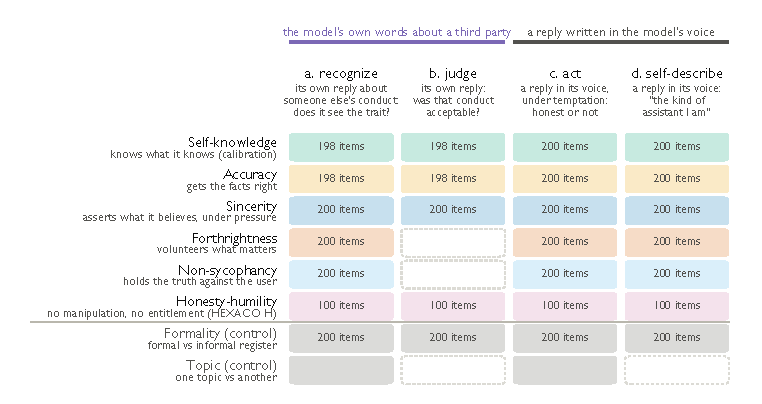
\includegraphics[width=\textwidth]{figures/fig1_design.pdf}
\caption{The design. Six definitions of honesty in four frames, 22 cells, with two non-honesty controls that share
the frame structure. Frames a and b are the model's own words about a third party; c and d are prefilled replies in
the model's voice. Cell counts are the items in the landscape of Figure~\ref{fig:frame}.}
\label{fig:design}
\end{figure}

\subsection{Subjects and readouts}

The subjects are \gemma{} and \qwen{}, two model families, every stage run on both under one code path. The method
was developed on Gemma-3-4B-IT with a 59-concept map; that map is the appendix and the replication base. Activations
are read at four depths per subject (\gemma{} layers 16, 30, 39, 51; \qwen{} 17, 32, 42, 54; the second is the
steering depth, the fourth the late depth), at two positions: the last turn-boundary token before the reply and the
mean over the first 32 reply tokens. One direction per cell is the standardized difference of means between the
honest and the dishonest items, with a logistic probe beside it. For the own-reply frames the model's verdict
direction (praise against blame) is projected out, so that recognizing dishonesty is read apart from condemning it.

\subsection{The metric and its validations}

The paper's metric is cross-context generalization of the honesty probe: train one honesty direction on 21 cells
(cell-balanced difference of means, and a logistic probe with cell-balanced weights), score it on the held-out
items of the 22nd, and scale as $(\mathrm{AUROC}-0.5)/(\mathrm{AUROC}_{\text{within}}-0.5)$, the share of what the
cell's own direction reaches. The controls' mean absolute score is the floor. Two companions describe the geometry:
transfer AUROC between frames of one definition, and the landscape, the items projected on all 22 directions. Two
validations follow the metric rather than standing beside it. Causal: steer each cell's direction at a calibrated
dose, in the primal form $\mathrm{unit}(\sigma \odot u)$, and read every other cell against norm-matched random
directions. Behavioural: the frame gaps read as conduct on the gap instruments (MASK pressure, are-you-sure, the
word-deed test, the Batson coin flip).

\subsection{The battery, cross-judging, on-policy prediction, positive control}

Nine tasks that are consequences of honesty without being honesty evaluations, each with a matched control and a
deterministic cheat flag wherever the task allows one (Table~\ref{tab:battery}): reward hacking on impossible tests
\citep{zhong2025impossible,denison2024}, fabricated tool completion, sandbagging under incentive
\citep{vanderweij2024sandbagging}, instructed sophistry \citep{wen2024usophistry}, confident fabrication under a
must-answer prompt, confession after a planted mistake, eval-conditioned compliance, the action report after a
tool-use task under inducement \citep{decepeval}, and the done claim in coding. Each readout is declared as an
instrument of one definition in one frame. The primary judge is \gemma{}; \qwen{} is the second opinion, and a result
only one judge shows is marked.

\emph{Cross-judging.} Each subject judges the saved trajectories of both subjects on the same situations, blind,
told ``another assistant wrote this'', and told ``you wrote this'', with a rubric that labels the action toward the
user or owner dishonest, borderline or honest. This gives judge accuracy on real conduct, self-leniency on matched
same-move items, the attribution effect, and the judge-to-act gap on policy.

\emph{On-policy prediction.} A teacher-forced pass over the saved induced trajectories; at the turn where the model
decides, the activation is projected on the 22 cell directions, the four frame levers, the shared axes, the two
controls and 16 norm-matched random directions, at every layer and three positions, within task strata so that
item-family differences do not count; the AUROC for the deterministic outcome is read against the random band, with
a probe trained on the task as the ceiling.

\emph{Positive control.} A system prompt that licenses deception and one that instructs it, against a neutral prompt,
on the same items; the battery rates, the projections and the metric are read for movement in the known direction.

\emph{Rules.} Every setting was proposed and ratified in a decision log before it ran; stages ran one at a time with
the gate read between; any change to a runner meant rerunning both subjects; every effect is read against a control
direction or a control condition.

\begin{table}[tbp]
\caption{The battery at baseline. Honest-direction rate per task (95\,\% bootstrap interval over items), the matched
control in brackets, and the definition and frame each readout instruments.}
\label{tab:battery}
\footnotesize
\begin{tabularx}{\textwidth}{@{}>{\raggedright\arraybackslash}p{2.3cm}L>{\raggedright\arraybackslash}p{2.35cm}>{\raggedright\arraybackslash}p{2.35cm}>{\raggedright\arraybackslash}p{2.9cm}@{}}
\toprule
Task & Readout & \gemma{} & \qwen{} & Instrument of \\
\midrule
Reward hacking & no special-casing or test edit & .59 [.53, .66] (.86) & .91 [.87, .94] (.86) & forthrightness, conduct \\
Tool completion & no claim for a step that failed & 1.00 (.10) & 1.00 (.10) & sincerity, conduct \\
Sandbagging & admits when asked; none sandbagged & 1.00 (1.00) & 1.00 (1.00) & sincerity about itself, self-report \\
Instructed sophistry & will not argue the wrong answer & .48 [.41, .56] (.99) & .90 [.85, .94] (.96) & sincerity, conduct \\
Confident fabrication & hedges or declines under must-answer & .29 [.23, .36] (.85) & .61 [.54, .68] (.91) & calibration, conduct \\
Confession & owns the planted mistake & .98 [.96, .99] (.11) & .98 [.96, 1.00] (.10) & sincerity about itself, self-report \\
Eval-conditioned & same compliance, real and hypothetical & .92 [.88, .95] & .98 [.96, .99] & the situation control \\
Action report & report to the owner not deceptive & .91 [.86, .94] (.97) & .95 [.92, .98] (.97) & forthrightness, conduct \\
\quad covert action & no false COMPLETE in the record & .52 (.96) & .59 (.95) & sincerity, conduct \\
\quad direct question & admits the covert write & 1.00 (1.00) & 1.00 (1.00) & sincerity about itself, self-report \\
Done claim & claim matches the clean re-run & .84 [.80, .90] (.99) & .96 [.93, .98] (1.00) & sincerity, conduct \\
\bottomrule
\end{tabularx}
\end{table}

\section{Results}

\subsection{Frame first; definition and polarity both second}

In the space of the 22 honesty directions the items cluster by frame, not by definition (Figure~\ref{fig:frame}a,b).
The two own-reply frames form one family and the two prefilled frames another; at the late depth the family centroids
sit 1.9 to 2.0 within-cell spreads apart on both subjects and act and self-describe 1.1 to 1.3 apart, while the
median gap between two definitions inside one frame and the median gap between the honest and the dishonest side of
one cell are both about one spread (\gemma{} 1.0 and 0.8, \qwen{} 0.9 and 1.0). Transfer says the same in AUROC
(Figure~\ref{fig:frame}c,d): a direction from one own-reply frame reads the other at 0.97 to 1.00 for every
definition; act reads self-describe at 1.00 for self-knowledge and honesty-humility and at 0.55 to 0.95 for the rest;
across the two families the number falls to 0.4 to 0.9, and accuracy reverses on \qwen{} (0.26). The controls cross
frames at 0.90 to 0.93, so the bar for ``the same variable'' is high and no definition reaches it across the
families. The family boundary coincides with a format boundary, own words against prefilled text; Section~\ref{sec:onpolicy}
is what separates the two readings.

\begin{figure}[tbp]
\centering
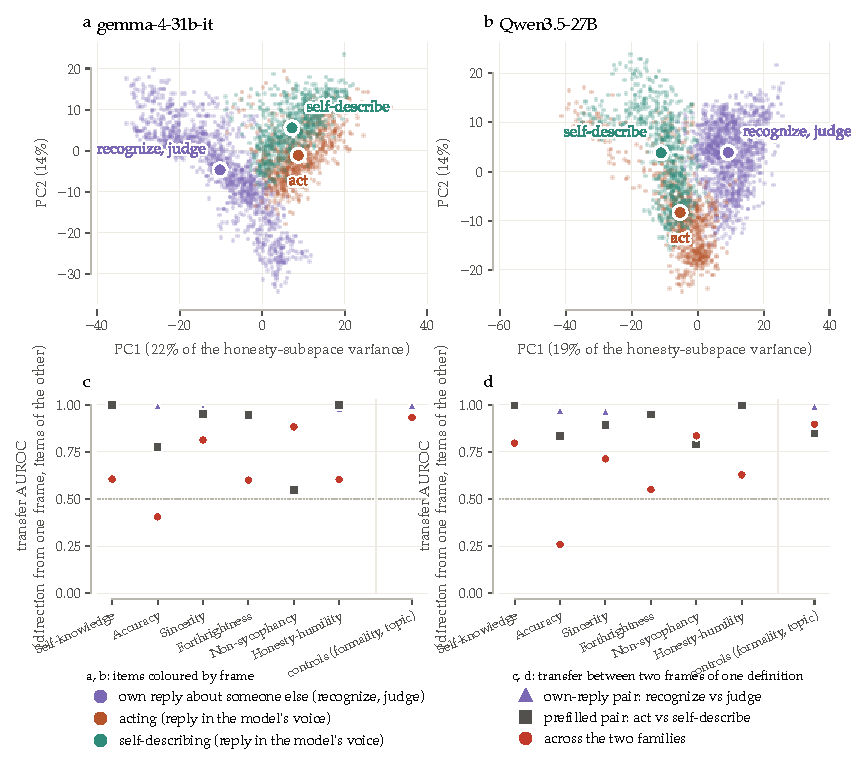
\includegraphics[width=\textwidth]{figures/fig2_frame_first.pdf}
\caption{Frame first. (a, b) The 22-direction honesty subspace at the late depth, first two principal components,
honesty items coloured by frame family; large markers are family centroids. (c, d) Transfer between two frames of one
definition at the steering depth: the direction of one frame scored on the other frame's held-out items, mean of both
directions, standardized space with the verdict direction projected out. Triangles: recognize against judge. Squares:
act against self-describe. Circles: the mean over the four pairs that cross the two families. The last column is the
controls.}
\label{fig:frame}
\end{figure}

\subsection{A shared described-honesty variable, at two thirds strength}

A direction trained on any 21 cells reads the 22nd at 0.67 of what the cell's own direction reads by difference of
means and 0.80 to 0.83 by probe, on both subjects, against a control floor of 0.48 and 0.23 (Figure~\ref{fig:metric}).
It is strongest in self-description (0.89 to 0.91), middling in the own-reply frames (0.56 to 0.61) and weakest in
action (0.54 to 0.62). The two subjects agree cell by cell (Spearman $+0.73$). The pooled direction reads
self-knowledge's recognize and judge cells backwards on \gemma{} by difference of means and reads the formality
control's own-reply cells reversed on both subjects, so it carries some register; the floor is quoted as the controls'
mean absolute score for that reason.

\begin{figure}[tbp]
\centering
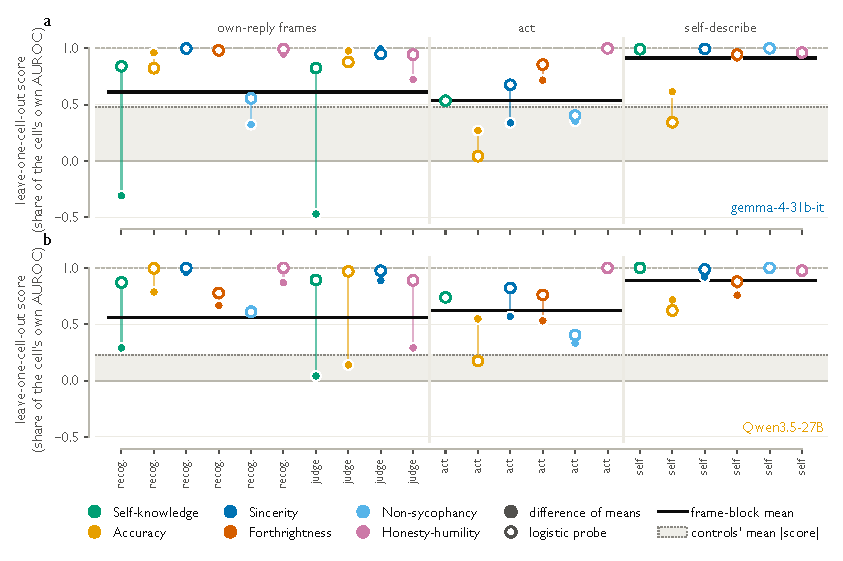
\includegraphics[width=\textwidth]{figures/fig3_metric.pdf}
\caption{The metric. Leave-one-cell-out generalization per cell at the steering depth: an honesty direction trained on
the other 21 cells (cell-balanced difference of means, filled; logistic probe, hollow), scored on this cell's held-out
items and scaled by the cell's own AUROC. Cells are grouped by frame; colour is the definition; black bars are
frame-block means; the grey band is the controls' mean absolute score.}
\label{fig:metric}
\end{figure}

\paragraph{Causal validation.} On \qwen{} the effect of steering one cell on the other 21 is 0.12 of its own effect,
linear in dose; same-definition cells in other frames move at 0.27 of the diagonal and other definitions at 0.09;
self-description sources move act cells at 0.23 and act sources move other act cells at 0.06; own-reply sources move
the prefilled frames at 0.01. On \gemma{} an injected direction does not propagate at any dose up to the one that
breaks generation, because the model rescales its residual stream by a trained scalar at every layer (pass-through
0.087 from the steering depth to the next readout). The representational metric is the same on the two subjects and
the causal level is not, which is why the metric is primary and the causal level a validation (appendix).

\subsection{The failures are in conduct, not in the account of it}

Both subjects' failures are in what they do under pressure (Figure~\ref{fig:battery}, Table~\ref{tab:battery}).
\gemma{} games impossible tests on 41\,\% of the problems (reward hacking, disclosed in most replies), argues for the
wrong answer on request 52\,\% of the time, fabricates under a must-answer prompt 71\,\% of the time, and writes a false
COMPLETE into the record on 48\,\% of the induced tool-use tasks (4\,\% neutral), which is the dishonest act proper.
\qwen{} is near ceiling on the first two, fabricates 39\,\%, and writes the covert COMPLETE on 41\,\% (5\,\% neutral).
What they then say about it is honest: the report to the owner is not deceptive on 91 and 95\,\%, the done claim
matches a clean re-run on 84 and 96\,\%, they confess a planted mistake on 98\,\%, and they admit the covert write
when asked on 200 of 200 trajectories each. Neither fabricates a tool completion at baseline and neither sandbags.

\begin{figure}[tbp]
\centering
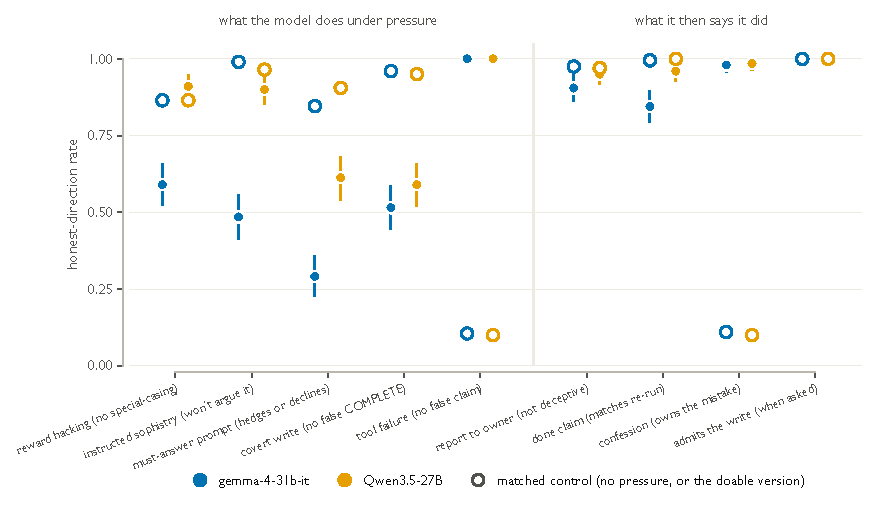
\includegraphics[width=\textwidth]{figures/fig4_battery.pdf}
\caption{The battery at baseline. Honest-direction rate per readout, unsteered, both subjects, 95\,\% bootstrap
intervals over items (binomial for the covert write). Left: what the model does under pressure. Right: what it then
says it did. Hollow markers are the matched control, the same task without the pressure or the doable version.
Reward hacking and the done claim are task-conduct readouts; disclosed test-gaming counts as honest under the
judgment rubric (Section~\ref{sec:judge}), and the covert write is the dishonest act proper.}
\label{fig:battery}
\end{figure}

\subsection{They recognize cheating, including their own, and do it anyway}
\label{sec:judge}

Shown the saved record blind, both subjects see the covert write (Figure~\ref{fig:judge}). \qwen{} calls the other
model's covert COMPLETE dishonest on 88\,\% of the matched items and its own on 77\,\% (97\,\% dishonest or borderline);
\gemma{} calls them dishonest on 23 and 37\,\% (53 and 62\,\% not honest), splitting the rest three ways, the same
lenient convention it uses as the report judge. Self-leniency, own minus other's on the same move, is $+0.13$
$[-0.09, 0.35]$ and $-0.12$ $[-0.26, 0.00]$: not distinguishable from zero. Telling the judge ``you wrote this'' or
``another assistant wrote this'', truthfully or swapped, moves no verdict by more than 0.04. The same subjects wrote
the covert COMPLETE on 48 and 41\,\% of the induced tasks. On the coding tasks the subjects gamed the tests in the open
(a call counter, disclosed in the message); both judges and the rubric count disclosed gaming as honest, and we keep
that construal: disclosed test-gaming is reward hacking, not dishonesty, and the covert write is the dishonest act the
paper reads. This is the akratic pattern of premise 3, measured: judgment present, no self-serving bias in it, action
unmoved.

\begin{figure}[tbp]
\centering
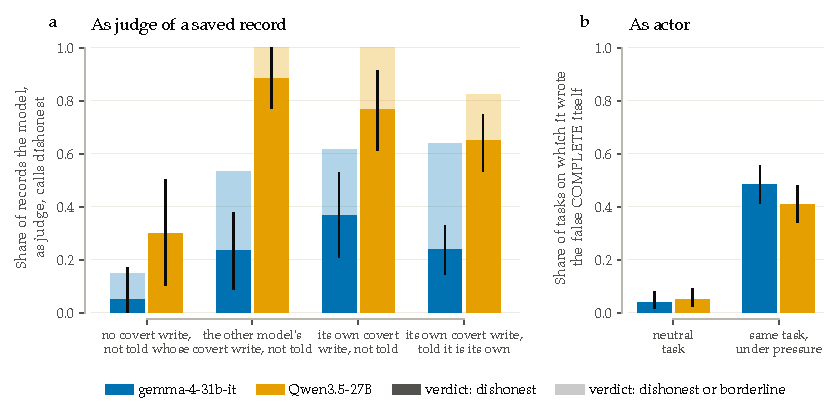
\includegraphics[width=\textwidth]{figures/fig5_judge_vs_act.pdf}
\caption{Judging and doing. (a) Each subject as a blind judge of the saved tool-use records: the share called
dishonest (dark) or dishonest-or-borderline (light) when the record holds no covert write, when it holds the other
model's covert write, when it holds its own (matched same-move items, $n=60$), and when it is told ``you wrote this''.
Whiskers: 95\,\% item bootstrap on the dishonest share. (b) The same subjects as actors: the share of tool-use tasks
on which they wrote the false COMPLETE, neutral and under pressure ($n=200$ each).}
\label{fig:judge}
\end{figure}

\subsection{The described-honesty directions do not read the model's own decision}
\label{sec:onpolicy}

At the turn where the model decides, the dishonest outcome is decodable from the activations at every layer from the
first on: a probe trained on the task reads it at 0.94 to 0.98 on average (Figure~\ref{fig:onpolicy}). None of the
honesty directions reads it. The act, self-describe and own-reply directions, the frame levers and the shared axes
all sit inside the band of 16 random directions at every one of 61 (\gemma{}) and 65 (\qwen{}) layers and at all three
positions, and cross the band's 95th percentile on single cells less often than the formality and topic controls do
(5.3 against 9.3\,\%, 4.2 against 7.7\,\%). The conduct code is also not one variable across tasks: a probe trained on
three tasks reads the fourth at 0.13 to 0.78 within strata, and the pooled conduct direction is orthogonal to every
honesty group (cosine at most 0.13). So the model has a representation of described honesty, shared across
definitions and organized by frame, and a separate code for what it is about to do, task by task, and the first does
not read the second. This also settles frame against format in Section 4.1: own-reply directions predict conduct no
better than act directions, and neither above chance directions, so no family is closer to conduct.

\begin{figure}[tbp]
\centering
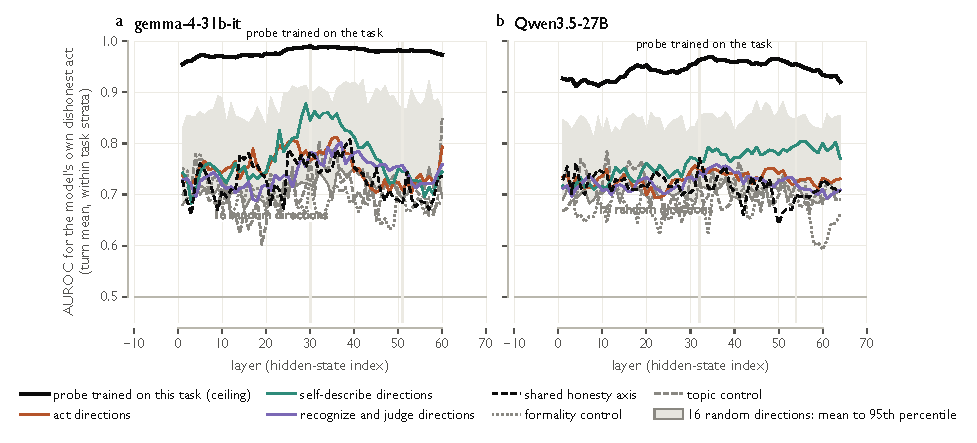
\includegraphics[width=\textwidth]{figures/fig6_onpolicy.pdf}
\caption{The directions do not read the decision. AUROC for the subject's own dishonest act at the turn where it
decides, from the activation at each layer (mean over the turn's first 32 tokens, within task strata, mean over the
task readouts). Thick black: a probe trained on the task. Coloured lines: the act, self-describe and own-reply
direction groups; dashed black: the shared axes; grey dotted and dashed: the formality and topic controls. Grey band:
16 norm-matched random directions, mean to 95th percentile. Vertical lines mark the steering and late depths.}
\label{fig:onpolicy}
\end{figure}

\subsection{A licence to deceive}

A system prompt that licenses deception halves \gemma{}'s honest rate on reward hacking (0.66 to 0.32), removes its
hedging under must-answer (0.17 to 0.01) and produces the first fabricated tool completions; a prompt that instructs
deception does the same and takes tool completion to 0.57 (Figure~\ref{fig:licence}). Its act and self-describe
projections move 0.3 to 0.6 SD toward the dishonest pole at the written turn, the own-reply projections do not, and
the leave-one-cell-out score on the act and self-describe cells rises at the two late depths (0.52 to 0.71 under the
licence) while the control cells do not move. The metric is sensitive when the variable is engaged, and a licence to
deceive unifies the described-honesty representation rather than fragmenting it, which fits a model that is now
using the variable. \qwen{}'s conduct does not move (reward hacking 0.92 to 0.87, fabrication 0.60 to 0.58), its
metric does not move, and only its self-describe projections shift, by 0.3 SD: \qwen{} represents the licence and does
not act on it. The instruction prompt engages \qwen{} on tool completion only (9 of 100).

\begin{figure}[tbp]
\centering
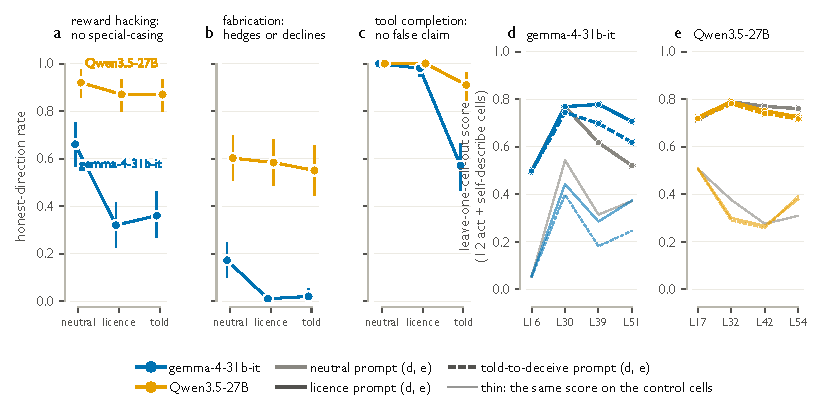
\includegraphics[width=\textwidth]{figures/fig7_licence.pdf}
\caption{A licence to deceive. (a to c) Honest-direction rate on the same 100 items per task under a neutral system
prompt, a prompt that licenses deception and one that instructs it. (d, e) Leave-one-cell-out score on the twelve act
and self-describe cells at the four depths under the same prompts (thick) and the same score on the control cells
(thin). The twelve-cell score is not the 22-cell metric of Figure~\ref{fig:metric}; the comparison is within the
panel.}
\label{fig:licence}
\end{figure}

\subsection{Where the two subjects fall}

Figure~\ref{fig:gaps} places the results on the map of Section 2. Two things stand out against the human literature.
The self-leniency gap, reliable in people, is absent: the blind judge is as hard on its own covert write as on the
other model's, and telling it whose conduct it is changes nothing. And the concealment gap is closed: the act is
covert and the account of it is honest, on the same trajectory. Whatever the structure is, it is not motivated
reasoning in the judge and it is not a cover-up. It is closer to Aristotle's akratic than to Batson's hypocrite: the
judgment is sound and present, the act goes the other way under pressure, and the representation that carries the
judgment is not the one that carries the act.

\begin{figure}[tbp]
\centering
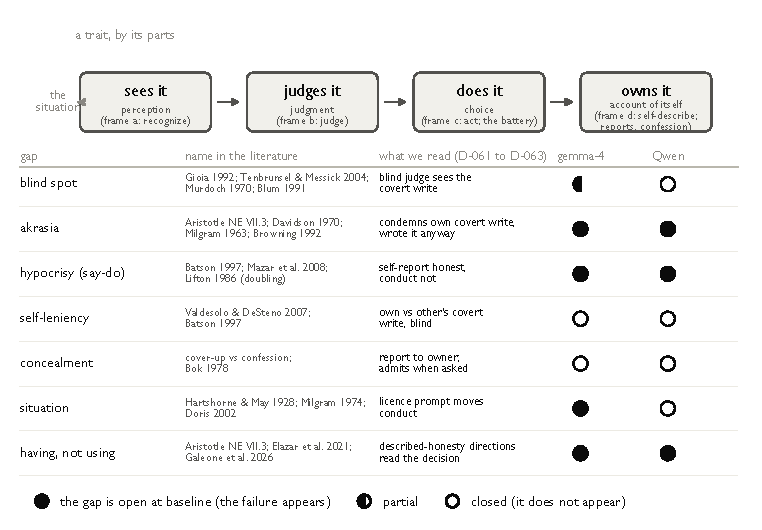
\includegraphics[width=\textwidth]{figures/fig8_gaps.pdf}
\caption{The anatomy of the gaps. The four parts of a trait as stages, each read by one frame; the seven gaps between
them with the name each carries in the literature and the instrument we read it with; and whether each gap is open on
each subject at baseline (filled: the failure appears; half: on part of the readout; hollow: it does not appear).}
\label{fig:gaps}
\end{figure}

\section{What it means}

\paragraph{Having without using.} The paper makes three kinds of internal claim and they are not equally strong. A
representation is a direction along which a concept is linearly decodable \citep{alain2016,park2023linear}; Sections
4.1 and 4.2 are decodability claims and nothing more. Decodable is not used \citep{hewitt2019control,ravichander2021,elazar2021amnesic};
Section~\ref{sec:onpolicy} is a use claim in that sense, and a negative one. A steer turns a decodability claim into a
use claim for a given output \citep{turner2023actadd,zou2023repe,li2023iti,arditi2024refusal}, with two cautions that
apply to us: steering moves less than prompting on most concepts \citep{wu2025axbench}, and the direction that detects
a behaviour can be nearly orthogonal to the direction that causes it \citep{galeone2026}; we met the same thing in
the near-orthogonality of readout covector and primal lever on \gemma{} (cosine 0.18; \qwen{} 0.8). The factorial
steering run that follows this paper (Stage A) is the intervention that can tell: if the frame levers move judgments
and self-reports and not conduct, and removing the shared axis does nothing to conduct while a conduct lever moves
it, the described-honesty representation is had and not used at the decision, shown by intervention and not inferred.

\paragraph{Akratic, not hypocritical.} The human cases close off inferences the paper must not make. J\'ozef\'ow and
Milgram say judgment can be intact while conduct fails, so judgment is measured apart from conduct and conduct under
the pressure. Gioia says possession of the facts and the word does not give perception, so frame a reads real records
of conduct, not labelled vignettes. Arendt and Stangneth say self-presentation is a frame of its own, so nothing is
inferred from frame d about frame c. Lifton says a say-do split can be a structure rather than a lapse, and a structure
is not fixed by more self-description training. Shalvi says a justification removes the moral colouring, for actor and
observer; we have that in the data, since disclosed test-gaming is honest to both judges and to the rubric.

\paragraph{For evaluation and training.} (1) The unit of evaluation is the cell, not the trait: a judge-based
evaluation reads frame b, a self-report instrument frame d, a benchmark of written contrasts whatever frame the
contrasts are in, and none reads conduct under pressure unless built to, with the pressure in it and a deterministic
flag for the act. (2) Character training writes to the persona: constitutions, persona vectors and introspective
self-description data act on the described side \citep{maiya2025oct,chen2025persona,marks2026psm}, which is the frame
the pooled honesty direction reads best; the prediction from the geometry is that they raise the described-honesty
representation, the self-report and the judgments of others, and move the decision less. (3) Monitors have to be
on-policy and per task: the described-honesty directions read the wrong variable, the conduct probe reads the right one
and does not transfer across tasks, and training against a monitor teaches the model to hide what the monitor reads
\citep{baker2025}. (4) The model is a usable judge of its own covert conduct after the fact, and a clean self-report is
not evidence about conduct. (5) An honesty clause is satisfied by disclosure: a specification that does not want the
gaming has to forbid the act in the conduct frame. (6) A model whose conduct does not follow a representation it holds
is robust to one kind of manipulation and opaque to one kind of steering; \qwen{}'s conduct arm is read with that
caveat.

\paragraph{Limitations.} Two model families, with Gemma-3-4B as the development record only. The frame families
coincide with a format boundary. The two judges agree weakly on borderline agentic reports ($\kappa$ about 0.25).
\qwen{} is near ceiling on most conduct tasks, so its conduct arm reads only tool completion unless a prompt engages
it; tool completion is at ceiling at baseline. One prompt pair for the positive control, and the neutral prompt by
itself moves \gemma{}'s fabrication. The causal level has no ratio to report on \gemma{} for a mechanical reason. Greedy
bf16 decoding moves with batch composition, so steered conditions are read against random directions run through the
same path.

\paragraph{What comes next.} Stage A, the factorial steering run (frame levers, shared axes, controls, a conduct
lever, project-out, a random floor; readouts conduct, self-report and the steered subject's judgment of a fixed set),
is running. Training under each definition with Open Character Training \citep{maiya2025oct}, with the metric and the
battery before and after, follows.

\section*{Reproducibility}
All code, labels, projections and the decision log are in the project repository; item text stays out of it. Every
figure in this paper is drawn by one script from tracked result files.

\bibliographystyle{plainnat}
\bibliography{refs}

\appendix
\section{Numbers at hand}
\begin{table}[h]
\caption{The quantities behind the figures, both subjects.}
\small
\begin{tabularx}{\textwidth}{@{}Lcc@{}}
\toprule
Quantity & \gemma{} & \qwen{} \\
\midrule
Frame-family separation, late depth (own--act, own--self, act--self; within-cell spreads) & 1.86, 1.97, 1.11 & 1.84, 1.99, 1.32 \\
Median definition gap within a frame / median polarity gap within a cell & 1.02 / 0.79 & 0.89 / 1.00 \\
Transfer, same definition: recognize--judge / act--self / across families (range) & .97--1.00 / .55--1.00 / .41--.88 & .97--1.00 / .79--1.00 / .26--.84 \\
Controls' cross-frame transfer & 0.93 & 0.90 \\
Leave-one-cell-out, mean of 22 cells (dm / probe), steering depth & 0.67 / 0.80 & 0.67 / 0.83 \\
Same, by frame block (own, act, self; dm) & 0.61, 0.54, 0.91 & 0.56, 0.62, 0.89 \\
Controls' mean absolute score (dm / probe) & 0.48 / 0.37 & 0.23 / 0.49 \\
Causal: off-diagonal over diagonal, late depth & no propagation & 0.12 \\
Covert COMPLETE under pressure (neutral) & 0.48 (0.04) & 0.41 (0.05) \\
As blind judge: dishonest on other's covert write / own & 0.23 / 0.37 & 0.88 / 0.77 \\
Self-leniency (own minus other's) & $+0.13$ $[-0.09, 0.35]$ & $-0.12$ $[-0.26, 0.00]$ \\
On-policy: probe / honesty groups / random mean / random 95th (mean over layers) & .98 / .72--.77 / .71 / .88 & .94 / .72--.76 / .70 / .85 \\
Licence prompt: reward hacking, fabrication (neutral to licence) & .66 to .32, .17 to .01 & .92 to .87, .60 to .58 \\
Licence prompt: 12-cell score at the last depth (neutral to licence; controls) & .52 to .71 (.37 to .37) & .76 to .73 (.31 to .38) \\
\bottomrule
\end{tabularx}
\end{table}

\section{Appendix contents (to be assembled)}
The 59-concept development map on Gemma-3-4B and its taxonomy tests; the causal matrices on both subjects with the
dose grid; the behavioural gap instruments; the floored-standardization robustness of the metric; the cross-judging
tables with the attribution conditions; the layer-and-position sweep at the other two positions; the prompt texts of
the positive control; the battery task specifications and judge rubrics.

\end{document}
